%programming realization

% \textcolor{red}{
% TODO: There must be an explanation of why we include it specifically in Fumili.
% Well, or it should appear in the previous part, where we've spoken about Fumili.
% }
Fumili, a package for minimizing the $\chi^2$-like functionals is one of the first minimizers included into ROOT release.
It has been showing it's reliability, stability and high convergence rate while it had been being used by scientific community for decades.

The greedy minimization algorithm which is employed in Fumili was first proposed at JINR by S.N. Sokolov~\cite{fum_1st} and developed by I.N.~Silin and V.S.~Kurbatov.
It linearizes the second derivatives, so the error matrix is always positively defined, and thus each step leads to a minimum.
Since Fumili is designed specifically to minimize $\chi^2$-like functionals, it finds a minimum faster and requires significantly fewer calls to the computationally intensive objective function than non-specialized minimization algorithms.

An implementation for the method of elimination of differentials has been designed as an extension of Fumili.
A corresponding class inherits from the ROOT class TFumili and adds the methods for setting constraints and their derivatives.

%очень общая схема включения дополнения в Fumili и ROOT
% \centering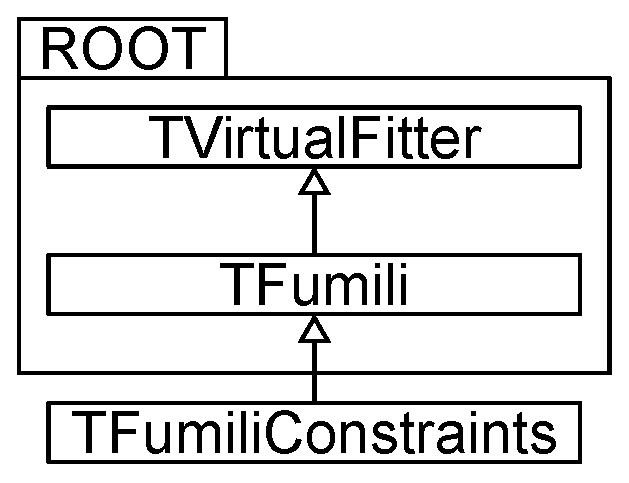
\includegraphics[width=0.4\textwidth]{pics/arch1.eps}

% \begin{figure}[htbp]
% \centering
% \centering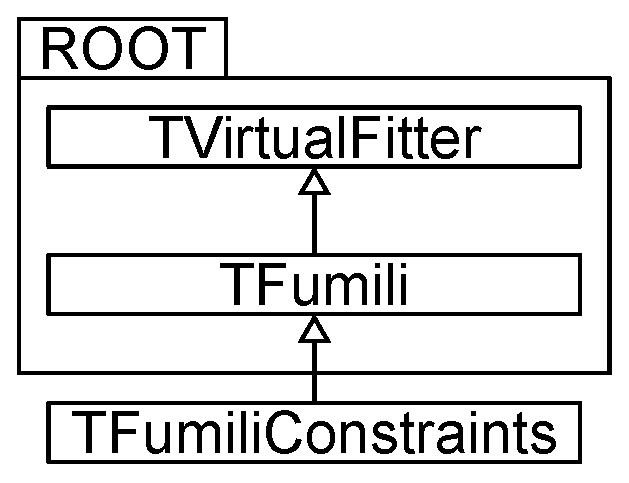
\includegraphics[width=0.35\textwidth]{pics/arch1.eps}
% \caption{
% Схема отношений классов при фитировании.
% Разработанный авторами класс TFumiliConstraints наследует от класса TFumili.
% }
% \label{arch}
% \end{figure}

%фактический user API. Несколько избыточен для статьи и вообще недоработан
% \begin{verbatim}
% void FCN(int & n_par, double * grad,
%          double & val, double * par, int flag);
% /* ... */
% TFumiliConstraints * fum = new TFumiliConstraints;
% // set parameters
% fum->SetParNumber(2);
% fum->SetParameter(0, "#alpha", .5, 0.01, 0, 0);
% fum->SetParameter(1, "#beta", .0, 0.01, 0, 0);
% // set constraints
% fum->SetConstrNumber(1);
% fum->SetConstraint(0, [](double * p){
%   return p[0]*p[0] + .5*p[1] - 1.3;
% });
% fum->SetConstrDeriv(0, 0, [](double * p){ return 2*p[0]; });
% fum->SetConstrDeriv(0, 1, .5);
% // set objective function
% fum->SetFCN(FCN);
% // minimize
% fum->Minimize();
%
% \end{verbatim}

